% ============================================================
%  Far From Here -- Apresentacao
%  Topicos Especiais em Computacao 2
%  Baseado no template "Beamer Template Universite Laval - Olico2 (monochrome)"
%  https://www.overleaf.com/latex/templates/beamer-template-universite-laval-olico2-monochrome/rfbnnjgbrpkx
% ============================================================

\documentclass[aspectratio=169]{beamer}

\usepackage[T1]{fontenc}
\usepackage[utf8]{inputenc}
\usepackage[brazil]{babel}
\usepackage{graphicx}
\usepackage{booktabs}
\usepackage{array}
\usepackage{xcolor}

\graphicspath{{figures/}}

% ---------- Paleta monocromatica ----------
\definecolor{ink}{HTML}{1A1A1A}
\definecolor{gray1}{HTML}{555555}
\definecolor{gray2}{HTML}{A0A0A0}
\definecolor{paper}{HTML}{FFFFFF}

\usetheme{default}
\setbeamertemplate{navigation symbols}{}
\setbeamerfont{frametitle}{size=\large,series=\bfseries}
\setbeamerfont{framesubtitle}{size=\small}
\setbeamercolor{normal text}{fg=ink,bg=paper}
\setbeamercolor{structure}{fg=ink}
\setbeamercolor{frametitle}{fg=ink,bg=paper}
\setbeamercolor{title}{fg=ink}
\setbeamercolor{subtitle}{fg=gray1}
\setbeamercolor{author}{fg=gray1}
\setbeamercolor{institute}{fg=gray1}
\setbeamercolor{date}{fg=gray1}
\setbeamercolor{itemize item}{fg=gray1}
\setbeamercolor{itemize subitem}{fg=gray2}
\setbeamercolor{section in head/foot}{fg=gray1,bg=paper}
\setbeamercolor{author in head/foot}{fg=gray2,bg=paper}
\setbeamercolor{title in head/foot}{fg=gray2,bg=paper}
\setbeamercolor{date in head/foot}{fg=gray2,bg=paper}
\setbeamertemplate{itemize item}{\raisebox{0.15ex}{\small$\bullet$}}
\setbeamertemplate{itemize subitem}{--}
\setbeamerfont{section in toc}{size=\small}
\setbeamertemplate{section in toc}{%
  \leavevmode\inserttocsection\par\vspace{0.2em}}

% ---------- Cabecalho: secao atual ----------
\setbeamertemplate{headline}{%
  \leavevmode%
  \vspace{2.2pt}%
  \hbox to\paperwidth{\hspace*{1.4em}%
    \usebeamercolor[fg]{section in head/foot}\fontsize{8.5}{10}\selectfont\insertsection\strut\hfill}%
  \vspace{1pt}%
  {\color{gray2}\hrule height 0.4pt}%
}

% ---------- Rodape: autor / titulo / pagina ----------
\setbeamertemplate{footline}{%
  \leavevmode%
  {\color{gray2}\hrule height 0.4pt}%
  \vspace{1pt}%
  \hbox{%
    \begin{beamercolorbox}[wd=.34\paperwidth,ht=2.4ex,dp=1ex,leftskip=1.4em]{author in head/foot}%
      \usebeamercolor[fg]{author in head/foot}\fontsize{8}{9}\selectfont\insertshortauthor
    \end{beamercolorbox}%
    \begin{beamercolorbox}[wd=.42\paperwidth,ht=2.4ex,dp=1ex,center]{title in head/foot}%
      \usebeamercolor[fg]{title in head/foot}\fontsize{8}{9}\selectfont\insertshorttitle
    \end{beamercolorbox}%
    \begin{beamercolorbox}[wd=.24\paperwidth,ht=2.4ex,dp=1ex,rightskip=1.4em]{date in head/foot}%
      \usebeamercolor[fg]{date in head/foot}\fontsize{8}{9}\selectfont\insertframenumber\,/\,\inserttotalframenumber
    \end{beamercolorbox}%
  }%
}

% ---------- Titulo ----------
\title[Far From Here]{Far From Here}
\author[Gabriel S. Lima]{Gabriel Dos Santos Lima}
\institute[UEA/EST]{%
  Universidade do Estado do Amazonas (UEA) \\
  Escola Superior de Tecnologia (EST) \\[1mm]
  \textbf{Disciplina:} T\'opicos Especiais em Computa\c{c}\~ao 2 \\
  \textbf{Prof.:} Jucimar Maia da Silva J\'unior%
}
\date{2026}

\begin{document}

\sloppy

% ============================================================
%  Pagina de titulo
% ============================================================
\begin{frame}[label=titulo, plain]
  \titlepage
  \begin{center}
    
\includegraphics[height=1.7cm]{uea_logo.png}
  \end{center}
\end{frame}

% ============================================================
%  Sumario
% ============================================================
\begin{frame}[label=toc]{Sum\'ario}
  \vspace{-1.6em}%
  \setlength{\leftskip}{4cm}%
  \footnotesize
  \tableofcontents[subsectionstyle=hide]
\end{frame}

% ============================================================
\section{Sobre o jogo}
% ============================================================
\begin{frame}{Sobre o jogo}
  \begin{columns}[T]
    \begin{column}{0.60\textwidth}
      \textbf{Far From Here} \'e um \textbf{roguelike de a\c{c}\~ao naval (PvE)},
      em vis\~ao \emph{top-down}, 2D pixelado, desenvolvido na
      \textbf{Godot 4.7} com GDScript.

      \medskip
      Voc\^e encarna o \textbf{Capit\~ao Piteu}, um pirata lend\'ario
      acometido por uma sonol\^encia m\'istica incontrol\'avel --- a
      \emph{N\'ovoa de Morfeu}.

      \medskip
      O pilar do jogo \'e o contraste entre o \textbf{combate ca\'otico de
      canh\~oes} e a \textbf{gest\~ao da fadiga/energia} do protagonista,
      que pode simplesmente \textbf{adormecer} em plena batalha.
    \end{column}
    \begin{column}{0.36\textwidth}
      \begin{center}
        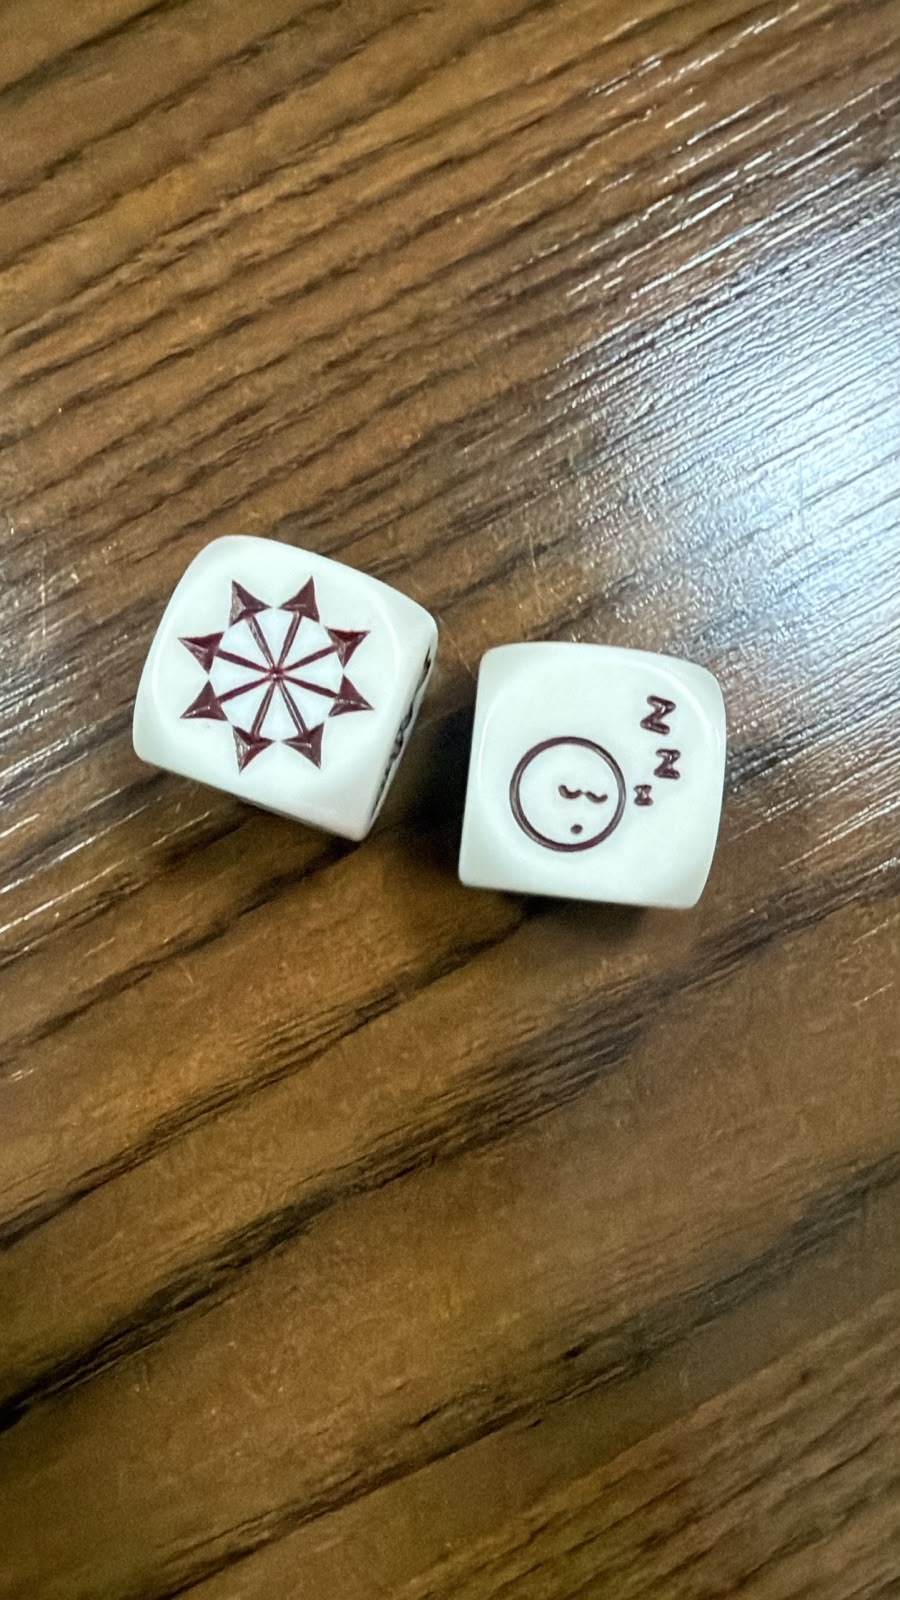
\includegraphics[height=0.56\textheight]{referencia.jpeg}\\[2mm]
        {\scriptsize Dados-tema: o \textbf{tim\~ao} e o \textbf{sono (Zzz)}
        --- as ideias centrais do jogo.}
      \end{center}
    \end{column}
  \end{columns}
\end{frame}

% ============================================================
\section{Hist\'oria}
% ============================================================
\begin{frame}{Hist\'oria}
  O lend\'ario pirata \textbf{Capit\~ao Piteu} acumulou tesouros incalcul\'aveis
  em anos de pilhagem, mas foi atingido por uma maldi\c{c}\~ao ancestral: a
  \textbf{N\'ovoa de Morfeu}, uma sonol\^encia m\'istica incontrol\'avel.

  \medskip
  A caminho da aposentadoria, ele adentrou o \textbf{Mar Ancestral}, dominado
  pela \textbf{Frota Espectral} --- piratas mortos-vivos que, aproveitando seus
  acessos de sono profundo, roubaram suas \textbf{rel\'iquias m\'agicas} e
  espalharam seu ouro pelo \textbf{Arquip\'elago dos Espectros}.

  \medskip
  Preso num ciclo infinito de n\'evoa e perigo, Piteu precisa afundar os navios
  assombrados, reunir as rel\'iquias e \textbf{romper o feiti\c{c}o}.
\end{frame}

\begin{frame}{A hist\'oria em 4 quadros}
  \begin{center}
    \vfill
    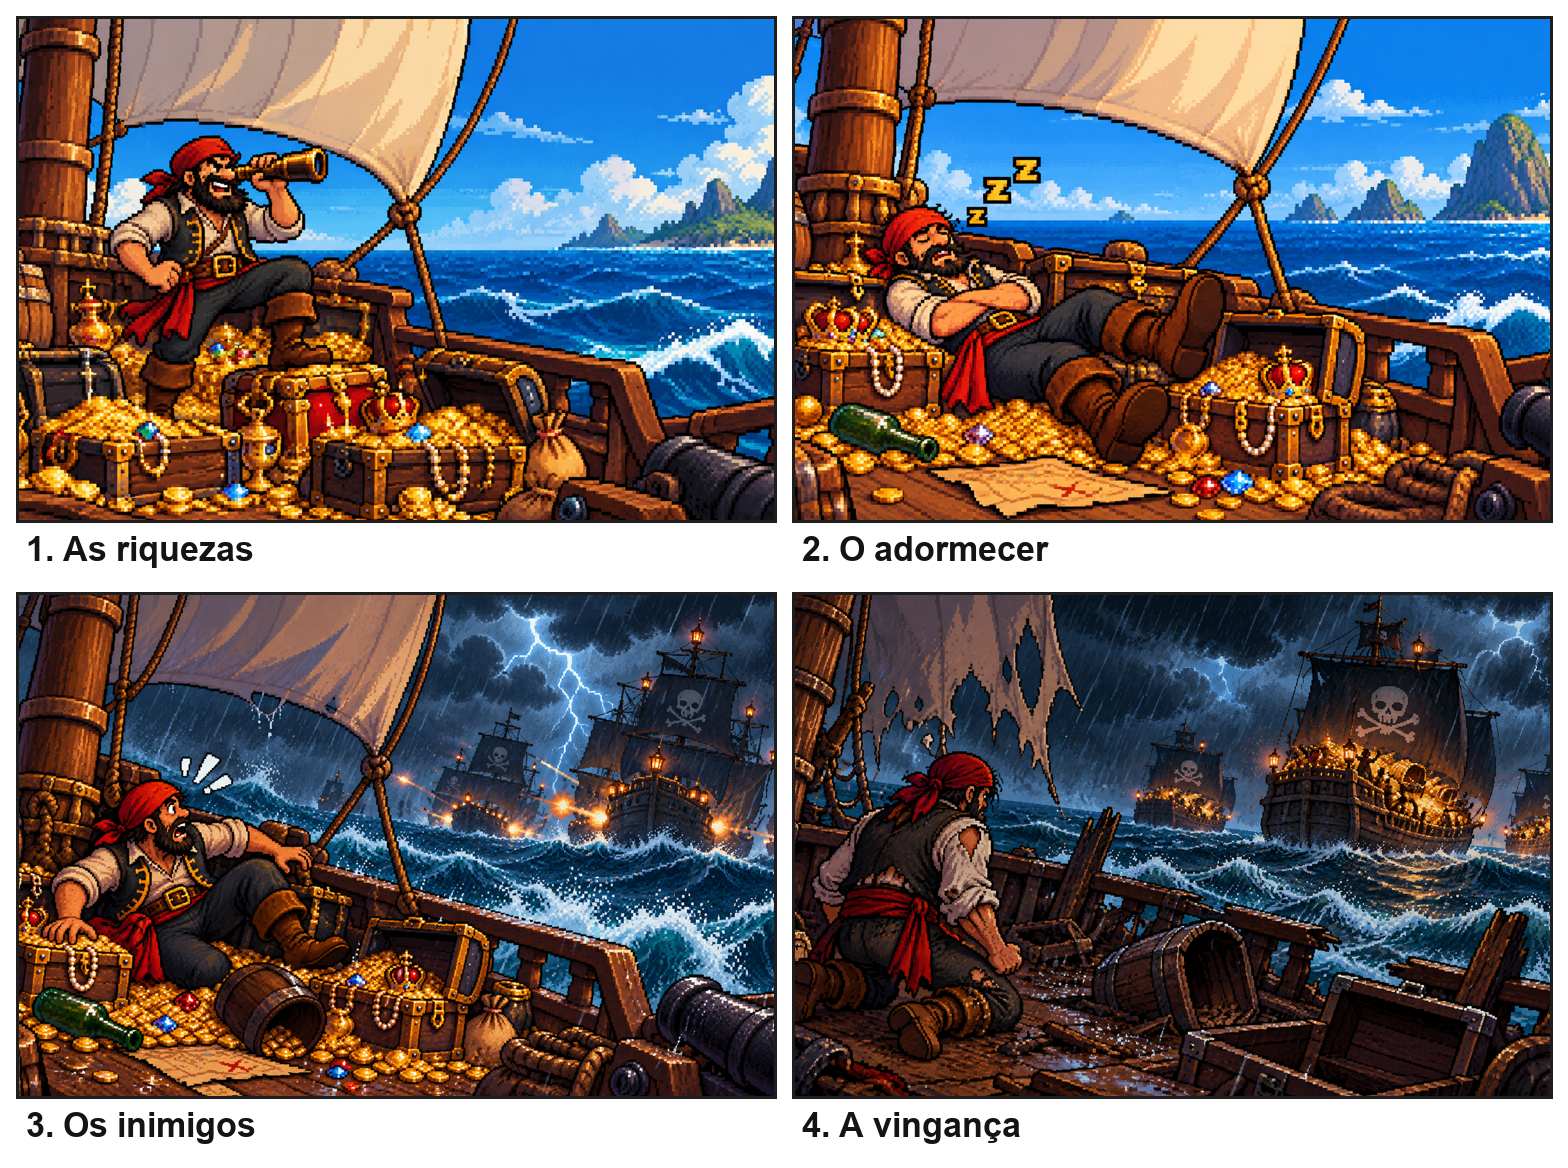
\includegraphics[width=0.58\textwidth]{historia_montagem.png}
    \vfill
  \end{center}
\end{frame}

% ============================================================
\section{Controles}
% ============================================================
\begin{frame}{Controles}
  \begin{columns}[T]
    \begin{column}{0.52\textwidth}
      \begin{table}
        \small
        \begin{tabular}{@{}ll@{}}
          \toprule
          \textbf{A\c{c}\~ao} & \textbf{Tecla} \\
          \midrule
          Acelerar (vela)      & \texttt{W} / $\uparrow$ \\
          Desacelerar / r\'e   & \texttt{S} / $\downarrow$ \\
          Bombordo (esquerda)  & \texttt{A} / $\leftarrow$ \\
          Estibordo (direita)  & \texttt{D} / $\rightarrow$ \\
          \textbf{Boost}       & \texttt{Shift} \\
          Mirar                & Mouse \\
          Atirar               & Bot\~ao esquerdo \\
          Som (mudo)           & \texttt{M} \\
          Avan\c{c}ar telas    & \texttt{Espa\c{c}o} / \texttt{Enter} \\
          \bottomrule
        \end{tabular}
      \end{table}
      \medskip
      {\small O jogador controla o \textbf{pr\'oprio navio}: vela, leme,
      mira e canh\~ao.}
    \end{column}
    \begin{column}{0.44\textwidth}
      \begin{center}
        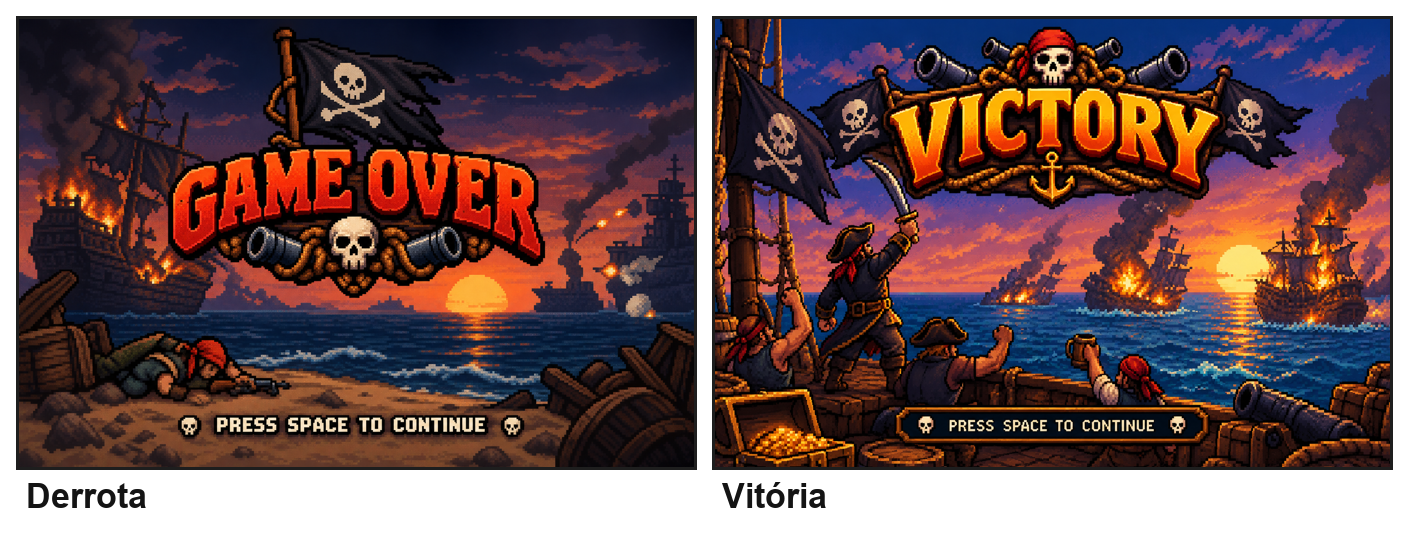
\includegraphics[width=\textwidth]{telas_montagem.png}\\[2mm]
        {\scriptsize As telas de \textbf{derrota} e \textbf{vit\'oria}
        fecham a partida.}
      \end{center}
    \end{column}
  \end{columns}
\end{frame}

% ============================================================
\section{Mec\^anicas}
% ============================================================
\begin{frame}{Mec\^anicas principais}
  \begin{itemize}
    \item \textbf{Energia, fadiga e sono (mec\^anica core):} o capit\~ao tem
      \textbf{10 de energia}; cada tiro custa \textbf{1} e a energia recarrega
      \textbf{1 ponto a cada 2 s}. Ao zerar, ele \textbf{dorme por 3 s} (im\'ovel,
      com o r\'otulo \textbf{``Zzz''}) e acorda recarregado.
    \item \textbf{Boost de velocidade:} \texttt{Shift} d\'a um pico de
      $\times 1{,}8$ por 2 s, ao custo de \textbf{5 de energia}.
    \item \textbf{Combate de canh\~ao:} proj\'eteis lentos com arco; uma
      \textbf{sombra marca o ponto de queda}, dando tempo de desviar
      (cad\^encia de 0,7 s). O boss dispara \textbf{3 canh\~oes} em leque.
    \item \textbf{Fogo:} de perto os espectros usam \textbf{lan\c{c}a-chamas} com
      queimadura; o boss enraivecido solta uma \textbf{explos\~ao radial de fogo}.
    \item \textbf{IA dos inimigos:} ficam inertes at\'e o jogador entrar no raio de
      detec\c{c}\~ao; ent\~ao perseguem, atiram e trocam para a
      \textbf{m\'usica de batalha}.
    \item \textbf{Vidas:} jogador e boss com \textbf{10 PV}, inimigos comuns com
      \textbf{3}. Afundar o jogador leva ao \textbf{game over}; destruir toda a
      frota leva \`a \textbf{vit\'oria}.
  \end{itemize}
\end{frame}

% ============================================================
\section{Interface (UI)}
% ============================================================
\begin{frame}{Interface (UI) e HUD}
  \begin{itemize}
    \item \textbf{Barras de status:} \textbf{vida} do jogador (verde) e
      \textbf{energia} (amarela), sempre vis\'iveis no canto superior esquerdo.
    \item \textbf{Barra do chefe:} aparece no topo apenas durante o combate
      contra o boss.
    \item \textbf{Minimapa:} jogador (verde), inimigos (vermelho), boss (magenta)
      e a \'area vis\'ivel da c\^amera (ret\^angulo branco).
    \item \textbf{Mira (crosshair):} desenhada na posi\c{c}\~ao do mouse, com o
      cursor do sistema \textbf{escondido} durante a fase.
    \item \textbf{Controle de \'audio:} bot\~ao de mudo e slider de volume no HUD.
    \item \textbf{Telas:} cutscene inicial, menu, \textbf{game over} e
      \textbf{vit\'oria}, com transi\c{c}\~oes em \emph{fade}.
  \end{itemize}
\end{frame}

% ============================================================
\section{Implementa\c{c}\~ao}
% ============================================================
\begin{frame}{Implementa\c{c}\~ao e ferramentas de IA}
  \begin{block}{Trilhas sonoras --- Google Gemini}
    M\'usicas-tema geradas para o menu, a navega\c{c}\~ao, a batalha, o game over
    e a cutscene, com \emph{crossfade} em tempo real.
  \end{block}
  \begin{block}{Imagens de cutscene --- ChatGPT}
    Os quatro quadros da hist\'oria e as telas de \textbf{game over} e
    \textbf{vit\'oria} foram gerados como imagens pixel-art.
  \end{block}
  \begin{block}{C\'odigo na Godot --- DeepSeek}
    Implementa\c{c}\~ao em \textbf{GDScript} (Godot 4.7): navios, canh\~oes,
    energia/sono, IA, HUD e transi\c{c}\~oes de cena, com apoio do DeepSeek.
  \end{block}
  \medskip
  {\small \textbf{Assets visuais:} sprites do Kenney \emph{Pirate Pack} (CC0) e
  oceano de Zabin \& Leonard Pabin (CC-BY-SA 3.0).}
\end{frame}

% ============================================================
\section{Demonstra\c{c}\~ao}
% ============================================================
\begin{frame}{V\'ideo de demonstra\c{c}\~ao}
  \begin{columns}[c]
    \begin{column}{0.4\textwidth}
      \begin{center}
        
\includegraphics[width=\textwidth]{qrcode.png}
      \end{center}
    \end{column}
    \begin{column}{0.58\textwidth}
      \textbf{Assista ao gameplay completo:}
      \bigskip

      \href{https://www.youtube.com/watch?v=-SHhYtDIbFU}%
        {\texttt{https://www.youtube.com/watch?v=-SHhYtDIbFU}}

      \medskip
      {\small Aponte a c\^amera do celular para o QR Code ao lado.}
    \end{column}
  \end{columns}
\end{frame}

% ============================================================
%  Obrigado
% ============================================================
\begin{frame}[plain]
  \vfill
  \begin{center}
    {\Huge\bfseries Obrigado!}\\[6mm]
    {\large Gabriel Dos Santos Lima}\\[2mm]
    {\small T\'opicos Especiais em Computa\c{c}\~ao 2 --- Prof. Jucimar Maia da Silva J\'unior}\\[2mm]
    {\small Universidade do Estado do Amazonas --- Escola Superior de Tecnologia}\\[6mm]
    
\includegraphics[height=1.4cm]{uea_logo.png}
  \end{center}
  \vfill
\end{frame}

\end{document}
